%!TEX root = ../my_thesis.tex

\graphicspath{{main/chapter1/fig/}}

\chapter{Context and Objectives}
\label{chap:ctx}

This first chapter presents the context of the digital communication systems
with a transmitter, a channel and a receiver. The most common metrics used
in digital communications are also introduced.

In the second section, the channel model and the modulation used all along
the manuscript are detailed. A characterization of the signal-to-noise ratio is
given as well as the notion of probability at the output of the channel and the
demodulator. The third section introduces the most famous channel codes.

In the forth and fifth sections, two use cases are presented: the simulation and
the software-defined radio. The simulation enables the development, the
validation and the comparison of a coding scheme while the software-defined
radio is a radio communication system where components that have been
traditionally implemented in hardware are instead implemented by means of
software.

The last section gives the main objectives of the thesis.

\vspace*{\fill}
\minitoccustom
\vspace*{\fill}

\section{Digital Communication Systems}
\label{sec:ctx_digital_communication_systems}

\begin{figure}[htp]
  \centering
  \includegraphics{intro/com_chain/com_chain}
  \caption{Digital communication chain.}
  \label{fig:intro_com_chain}
\end{figure}

It is now commonplace to state that Humanity has entered the era of
communication. By 2025, there should be more than 5 billion smart-phones in
circulation worldwide. Moreover, all kinds of objects will increasingly also use
communication technology, to exchange information in the \emph{Internet of
Things} (IoT) for instance. Despite their variety, all communication systems are
based on a common abstract model proposed by Claude Shannon. In his seminal
paper~\cite{Shannon1948}, he proposed to model a communication system with five
components: an information source, a transmitter, a channel, a receiver and a
destination. This model was later refined as shown in
Figure~\ref{fig:intro_com_chain}. The source produces a digital message $\bm{u}$
to be transmitted (sequence of bits). The channel encoder transforms it in a
codeword $\bm{c}$ to make it more robust to errors. In order to make possible
the information transmission through the channel, it is necessary to shape the
data stream. For instance, in the case of wireless communication, this stream
must be represented by a high-frequency signal in order to be transmitted by a
reasonably sized antenna. This is the role of the digital modulator which
produces a vector of symbols $\bm{x}$. The channel alters the signal with some
noise and distortions ($\bm{y}$). On the receiver side, the components perform
the inverse operations to retrieve the message $\bm{\hat{u}}$ produced by the
source.

In channel coding, also known as \emph{forward error correction} (FEC), $K$
information bits  are encoded in the transmitter. It results in a codeword
$\bm{c}$ of $N$ bits. $P = N - K$ is the number of parity bits added as
redundant information and $R = K/N$ is the code rate. The higher the code rate
$R$ is, the lower the number of parity bits $P$ is. The performance of this
chain is measured by estimating the residual error rate at the sink. It is
possible to observe two different rates: 1) the Bit Error Rate (BER); 2) the
Frame Error Rate (FER). The BER is calculated considering the $K$ information
bits independently, for instance a $10^{-3}$ BER means that there is an average
of one binary error per thousand message bits transmitted. The FER is computed
considering the entire frame, if there is one, two or more wrong bits in the
current frame, it will be counted as one error frame. A $10^{-2}$ FER means that
there is an average of one frame error per hundred frame transmitted. These
rates depend on many factors: the noise of the channel, the modulation
type, the code type, the code rate $R$, etc. The lower the bit and frame error
rates are, the higher the correction power of the system is.

\section{Channel Model}

In this thesis, only causal transmission channels without memory effect and
stationary are considered. In other words, the output of the channel at time $t$
only depends on its input at time $t$. In order to describe the disturbance
applied to the message $\bm{x}$ passing through the transmission channel,
different models can be used. However, in the literature, the selected model is
often the Additive White Gaussian Noise (AWGN) channel. In particular, this
channel well models the thermal noise which is one of the sources of noise
always present on the receiver side. This section presents the AWGN channel
concepts and introduces the Binary Phase-Shift Keying modulation/demodulation
that will be used all along the manuscript.

In the AWGN channel, the law binding the $y_i$ output to its $x_i$ input is of
the form $y_i = x_i + n_i$ with $N_{chn}$ an independent and identically
distributed variable according to a normal (or Gaussian) law centered in zero
and of variance $\sigma^2 = N_0 / 2$. So, we have $N_{chn} \simeq \mathcal{N}(0,
\sigma^2)$ and:
\begin{equation}
P_r(y_i|x_i) = \frac{1}{\sqrt{2\pi\sigma^2}}\exp{\Big(-\frac{(y_i-x_i)^2}{2\sigma^2}\Big)}.
\end{equation}

To estimate the correction power of a system it is very common to vary the
Signal-to-Noise Ratio (SNR). On the AWGN channel the SNR is generally given by
$E_b/N_0$ (in dB). $E_b$ corresponds to the average energy per information bit.
It can also be given by $E_s/N_0$ (in dB) where $E_s$ corresponds to the average
energy per transmitted symbol. A symbol is a waveform, it can be represented by
one or more bits. $E_s/N_0$ can be deduced from $E_b/N_0$:
\begin{equation}
\frac{E_s}{N_0} = \frac{E_b}{N_0} + 10.\log{(R.b_S)},
\end{equation}
where $R$ is the code rate and $b_S$ is the number of bits per transmitted
symbol $x_n$. $b_S$ depends on the modulation order, if a binary modulation is
used, then $b_S = 1$. The channel variance is:
\begin{equation}
\sigma = \sqrt{\frac{1}{2 \times 10^{\frac{E_s}{N_0} / 10}}}.
\end{equation}

An important characteristic of a channel is its capacity~\cite{Ryan2009}. The
capacity represents the maximal quantity of information that the canal can
transport. In other terms, it is impossible to find a coding scheme that
transports more information than the channel capacity.
From this capacity it is possible to deduce Shannon's limit~\cite{Shannon1948}.
This limit is the asymptotic SNR in $E_b/N_0$ (dB) which cannot be improved with
any channel code. When $R$ tends towards zero it can be shown that Shannon's
limit is $-1.59$ dB. This means that, for an AWGN channel, no system can
reliably transmit information at a SNR of less than $-1.59$ dB.

In the next chapters of the manuscript, the AWGN channel will mainly be
associated with a Binary Phase-Shift Keying (BPSK) modulation ($b_S = 1$). With
this modulation, each binary value $c_i \in \{0,1\}$ is associated to a real
value $x_i \in \{1,-1\}.$ The $\bm{l}$ outputs estimated by the digital
demodulator are given in the form of a Log Likelihood Ratio (LLR). Their sign
determines for each channel output data $y_i \in \bm{y}$ the most likely binary
input $c_i \in \bm{c}$. The absolute value corresponds to the degree of
reliability of the information. The mathematical expression for $l_i$ is:
\begin{equation*}
l_i = \log{\Big(\frac{P_r(y_i|c_i = 0)}{P_r(y_i|c_i = 1)}\Big)}.
\end{equation*}

\section{Capacity-approaching Channel Codes}

After Shannon, researchers have designed new coding/decoding schemes to approach
Shannon's theoretical limit increasingly closer. Indeed, recent progresses
managed to design practical codings performing very close to that limit, and are
already integrated in everyday communication systems. These code are usually
classified in two families: block codes and convolutional codes. The block codes
generate the redundancy by chunks of data while the convolutional codes compute
the redundancy in continue on the data stream. The purpose of this section is to
introduce to most famous channel code families.

The Turbo Product Codes (TPC) are block codes, they have been invented by Peter
Elias in 1954~\cite{Elias1954}. A TPC is the product of two block codes, it
results in a matrix where one code can be read from the columns and the other
one from the lines. The TPC are notably used in the WiMAX standard.

The Raj \textbf{B}ose, D. K. Ray-\textbf{C}haudhuri and Alexis,
\textbf{H}ocquenghem (BCH) codes are block codes discovered in the late
1950s~\cite{Hocquenghem1959,Bose1960}. They are algebraic codes built from a
polynomial. They are able to correct $T$ errors in a block of $N$ bits. These
codes are used in the CDs, DVDs and SSDs. In modern coding schemes, they are
often concatenated to other codes in order to improve the their correction power
especially when there is erroneous frames with a small number of erroneous bits
(this is the case in the DVB-S2 standard for instance).

The Irving S. \textbf{R}eed and Gustave \textbf{S}olomon (RS) codes have been
proposed in 1960~\cite{Reed1960}. Like the BCH codes they are built from a
polynomial but unlike the BCH codes, the RS codes are based on symbols instead
of bits (non-binary codes). The RS codes are used in many standards (CD, DVD,
Blu-ray, ADSL, DVB-T, etc.). If the number of bits per symbols is one, then the
RS codes are equivalent to the BCH codes.

The Low-Density Parity-Check (LDPC) codes are linear block codes, they have been
discovered very early by Robert G. Gallager in 1962~\cite{Gallager1962}.
Unfortunately, at the time of their discovery, the computational power available
in the transceivers was not sufficient to use them. But, in 1995, the LDPC codes
have been re-discovered by David MacKay~\cite{MacKay1995} and used in many
digital communication standards since (Wi-Fi, WiMAX, WRAN, 10Gbps Ethernet,
DVB-S2, CCSDS, 5G data transport, etc.).

The turbo codes have been discovered by Claude Berrou in 1993~\cite{Berrou1993}
and have been used in many digital wireless communication standards since (3G,
4G, DVB-RCS2, CCSDS, etc.). Unlike the LDPC codes, the turbo codes are
convolutional codes. The particularity of the turbo codes is to be composed by
two sub-codes. In other terms, the turbo codes are a parallel concatenation of
two convolutional codes.

The polar codes are linear block codes like the LDPC, they have been discovered
relatively recently by \Arikan in 2009~\cite{Arikan2009} and are used in the
5G standard (control channels). The particularity of these codes is that they
are the only ones for which it has been mathematically demonstrated that they
reach the Shannon's limit (considering an infinite codeword length).

Of course many other codes exist like the simple convolutional
codes~\cite{Elias1955}, the Reed-Muller codes~\cite{Muller1954,Reed1954}, the
raptor codes~\cite{Shokrollahi2004}, etc. The purpose of this section is not to
be exhaustive but to give a representative overview of the domain. This thesis
will focuses on a subset of these codes, namely the LDPC, the turbo and the
polar codes.

\section{Simulation}

There are many possible coding schemes with different characteristics. The
previous section presented different codes used in most of today standards.
Before they were standardized, these codes have been evaluated and compared.
The codes can be constructed in a infinity of different ways and for each coding
scheme, many different decoding algorithms can be implemented. It is then
mandatory to be able to evaluate and compare the BER/FER decoding performance of
the selected codes with each others before to implement them in real systems. To
this purpose, the channel coding specialists use simulation. Depending on the
channel model it is possible to predict with varying degrees of ease (in term of
computational effort) the BER/FER decoding performance of a communication
system. For simple channel models it is possible to evaluate analytically the
performance but when the channel model complexity increases it becomes
impossible to use direct methods. This is especially the case with the AWGN
channel presented before. The solution is then to resort to a compute intensive
Monte Carlo simulation of the communication system. The idea is to evaluate the
performance of the system by generating many random frames and applying random
noise samples on these frames, then the noisy frames are decoded and the output
sequence of bit $\bm{\hat{u}}$ is compared with the initial information bits
$\bm{u}$.

\begin{figure}[htp]
  \centering
  \subfloat[][Specification of the processing chain.]
  {
    \includegraphics[scale=1]{simu/com_chain/com_chain}
    \label{fig:simu_com_chain_specs}
  }
  \\
  \subfloat[][Input simulation parameters and output BER results.]
  {
    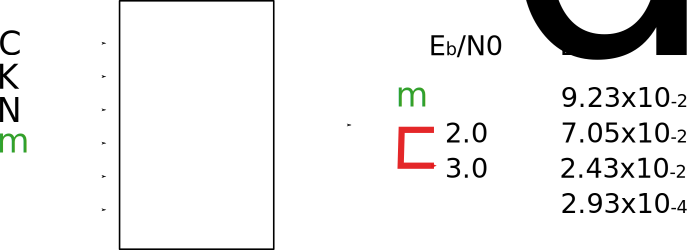
\includegraphics[scale=1]{simu/in_out/in_out}
    \label{fig:simu_com_chain_in_out}
  }
  \caption{Example of a digital communication system simulation.}
  \label{fig:simu_com_chain}
\end{figure}

Fig.~\ref{fig:simu_com_chain_specs} describes a processing sequence similar
to the digital communication chain presented in Fig.~\ref{fig:intro_com_chain}.
The only difference is that the \emph{sink} block has been replaced by what we
call a \emph{monitor}. The \emph{monitor}, unlike the \emph{sink}, knows the $K$
output information bits from the \emph{source} ($\bm{u}$). The $C$, $K$ and $N$
parameters are, respectively, the type of the code, the number of information
bits and the codeword size. These parameters have a direct impact on the
selection of the \emph{channel encoder} and the \emph{channel decoder} blocks
in the simulation. Fig.~\ref{fig:simu_com_chain_in_out} shows the BER output of
the simulation. The $m$, $M$ and $s$ parameters allow to control the AWGN
channel noise. $m$ is the minimum SNR value to simulate in the channel, while
$M$ is the maximum SNR value. $s$ is the SNR step between two SNR values.

\begin{figure}[htp]
  \centering
  \subfloat[][LDPC code ($R = 5/6$).                ]{\includegraphics[width=0.30\textwidth]{simu/bfer/bfer_ldpc}  \label{fig:intro_bfer_ldpc}}   \quad{}
  \subfloat[][Turbo code ($R \approx 1/3$).         ]{\includegraphics[width=0.30\textwidth]{simu/bfer/bfer_turbo} \label{fig:intro_bfer_turbo}}  \quad{}
  \subfloat[][Polar code ($R \approx 0.84$).        ]{\includegraphics[width=0.30\textwidth]{simu/bfer/bfer_polar} \label{fig:intro_bfer_polar}}  \\
  \subfloat[][Turbo product code ($R \approx 0.78$).]{\includegraphics[width=0.30\textwidth]{simu/bfer/bfer_tpc}   \label{fig:intro_bfer_tpc}}    \quad{}
  \subfloat[][Algebraic codes ($R \approx 0.93$).   ]{\includegraphics[width=0.30\textwidth]{simu/bfer/bfer_bch_rs}\label{fig:intro_bfer_bch_rs}} \quad{}
  \subfloat[][Convolutional codes ($R \approx 1/2)$.]{\includegraphics[width=0.30\textwidth]{simu/bfer/bfer_rsc}   \label{fig:intro_bfer_rsc}}
  \caption
    [BER and FER simulation results on various code families.]
    {BER and FER simulation results on various code families and decoder
    configurations. Lower is better. The codes are given in the $(N,K)$ form.}
  \label{fig:intro_bfer}
\end{figure}

As an illustration, Fig.~\ref{fig:intro_bfer} presents BER and FER decoding
performances estimated with Monte Carlo simulations on a large variety of code
families and decoding parameters. On each graphic, the BER is plotted with solid
lines while the FER is plotted with dashed lines. Both the BER and the FER
depend on the SNR ($E_b/N_0$). The higher the SNR is, the less there is noise
and therefore fewer errors. For instance, in Fig.~\ref{fig:intro_bfer_ldpc}, on
the same LDPC code ($N = 648$ and $K = 540$) and considering a 5.0 dB SNR, the
configuration 2 of the decoder achieves better decoding performance than the
configuration 1 because the {\color{Paired-3} green} curve is below the
{\color{Paired-7} orange} curve. In other terms, lower is better. Each time
there is two decoder configurations, the second one gives better BER/FER
decoding performance, this is achieved at the cost of a higher computational
effort compared to the first configuration. The purpose of
Fig.~\ref{fig:intro_bfer} is not to compare the codes with each others but to
introduce the typical BER/FER curves that will be used in the next chapters and
to show that there is a large set of possible combinations of codes and
parameters.

\section{Software-Defined Radio}

A cellular network or mobile network is a communication network where the last
link is wireless. The principle of mobile networks is to divide the territory
into zones called ``cells''. Each cell is associated to a base station and a
number of frequency channels to communicate with mobile terminals. Each base
station is connected to the networks handling voice calls, text messages and
Internet. As standards evolve, the structure of mobile networks changes in order
to increase throughput and latency performance and to increase the number of,
connected terminals. The objective is to cope with the exponential growth of
terminals.


\begin{figure}[htp]
  \centering
  \subfloat[][Traditional base station.]{\includegraphics[scale=0.715]{sdr/base_station/base_station_1G_2G} \label{fig:ctx_sdr_base_station_1G_2G}}
  \quad{}
  \subfloat[][BB and RF processing separation.]{\includegraphics[scale=0.715]{sdr/base_station/base_station_3G_4G} \label{fig:ctx_sdr_base_station_3G_4G}}
  \quad{}
  \subfloat[][Cloud-RAN]{\includegraphics[scale=0.715]{sdr/base_station/base_station_5G_future} \label{fig:ctx_sdr_base_station_5G_future}}
  \caption
    [Base stations evolution in mobile networks.]
    {Base stations evolution in mobile networks.}
  \label{fig:ctx_sdr_base_station}
\end{figure}

In the two first generations of mobile network (1G and 2G), all the signal
processing was treated in the base station near the antenna (cf.
Fig~\ref{fig:ctx_sdr_base_station_1G_2G}). Since the third generation of mobile
networks (3G) two types of processing have been separated: 1) the radio
frequency (RF) processing on the one side and 2) the base band (BB) processing
on the other side. The RF processing is attached to the antenna while the BB
processing is regrouped for multiple antennas (cf.
Fig~\ref{fig:ctx_sdr_base_station_3G_4G}). The range of this type of station is
approximately 40 kilometers. The connexions between the antennas and the BB
station are made through wired links. The RF processing mainly converts the
analog signal into a digital one (or the other way around) while the BB station
performs all the digital processing including the encoding/decoding and the
digital modulation/demodulation. The purpose of separation of the RF and BB
processing is to be able to put the BB stations near the urban centers and so to
facilitate their maintenance and to reduce the costs.

The virtualization of the mobile network is considered by industrial
actors~\cite{Huawei2013,Ericsson2015} and academic ones~\cite{Wubben2014,
Rost2014,Checko2015a} as a promising evolution. This is also known as the
\emph{Cloud Radio Access Network} (Cloud-RAN). The Cloud-RAN is especially
proposed for a part of the processing traditionally made in the base stations.
In this network structure, the computational hardware resources of the BB
processing are shared between multiple antennas (cf.
Fig~\ref{fig:ctx_sdr_base_station_5G_future}). This enables new optimizations:
1) better adaptation to non-uniform traffic; 2) energy saving; 3) throughput
increase and latency reduction; 4) increased scalability and
maintainability~\cite{Checko2015a}. To this purpose, the computational BB units
have to be virtualized: there should no longer be dedicated hardware to specific
antenna. On the contrary, the BB computational effort has to be distributed at
the cloud level. From the first to the forth generation of mobile networks, the
BB processing was systematically made on Application-Specific Integrated
Circuits (ASICs or dedicated hardware) but with the emergence of the Cloud-RAN
more flexible solutions like the software ones are seriously considered. On the
receiver side, the algorithms can be compute intensive (especially the digital
demodulation and the channel decoding). Knowing that, the challenge is to be
able to propose high throughput and low latency software implementations as well
as flexible ones~\cite{Nikaein2015,Rodriguez2017}. This is also known as the
\emph{Software-Defined Radio} (SDR).

\section{Objectives}

On the eve of the 5G mobile communication generation, the challenge is now to
design communication systems able to transmit huge amounts of data in a short
time, at a small energy cost, in a wide variety of environments. Researchers
work at refining existing coding schemes further, to get low residual error
rates with fast, flexible, low complexity decoders.

The validation of a coding scheme requires estimating its error rate
performance. Usually, no simple mathematical model exists to predict such
performance. The only practical solution is to perform a Monte Carlo simulation
of the whole chain: some data are randomly generated, encoded, modulated,
noised, decoded, and the performance is then estimated by measuring the Bit
Error Rate (BER) and the Frame Error Rate (FER) at the sink. This process leads
to three main problems:

\begin{enumerate}
  \item \textbf{Simulation time:}
    100 erroneous frames must be simulated to accurately estimate the FER/BER.
    Thus, measuring a FER of $10^{-7}$ requires simulating the transmission of
    $\sim100\times 10^7=10^9$ frames. Assuming a frame of 1000~bits, the
    simulator must then emulate the transmission of $10^{12}$~bits. Keeping in
    mind that the decoding algorithm complexity may be significant, several
    weeks or months may be required to accurately estimate the FER/BER of a
    coding scheme.

  \item \textbf{Algorithmic heterogeneity:} A large number of channel codes have
    been designed over time. For each kind of code, several decoding algorithms
    are available. While it is straightforward to describe a unique coding
    scheme, it is more challenging to have a unified software description that
    supports all the coding schemes and their associated algorithms. This
    difficulty comes from the heterogeneity of the data structure necessary to
    describe a channel code and the associated decoder: turbo codes use
    trellises, LDPC codes are well-defined on factor graphs and polar codes are
    efficiently decoded using binary trees.

  \item \textbf{Reproducibility:} It is usually tedious to reproduce results
    from the literature. This can be explained by the large amount of empirical
    parameters necessary to define one communication system, and the fact that
    not all of them are always reported in publications. Moreover, the simulator
    source codes are rarely publicly available. Consequently, a large amount of
    time is spent ``reinventing the wheel'' just to be able to compare to the
    state-of-the-art results.
\end{enumerate}

Moreover, new paradigms like the Cloud Radio Access Network (Cloud-RAN) and the
Software-Defined Radio (SDR) are now considered in real communication systems.
To match the real time constraints, here are the main challenges:

\begin{enumerate}
  \item \textbf{High throughput:} New applications, like the video streaming,
    can be very data-intensive, as a consequence, the compute intensive blocks
    of the transceiver have to be well optimized to reach levels of performance
    comparable with the hardware solutions.
  \item \textbf{Low latency:} Reaching high throughput is not always the major
    constraint, for instance, in audio-conferencing applications it is
    uncomfortable to perceive a delay when people are speaking.
  \item \textbf{Flexibility:} The software implementations have to be able to
    adapt to various configurations, for instance, when the SNR is changing,
    the code rate $R$ of the decoder can be switched on the fly.
\end{enumerate}

In this thesis we propose to study the most time consuming algorithms of digital
communication systems, to adapt and optimize them on General Purpose Processors
(GPPs) like the CPUs. The long simulation times and the real world application
requirements make it desirable to have \textbf{high throughput and low latency
implementations}. The algorithmic heterogeneity requires \textbf{flexible,
modular software}. The reproducibility issue pushes towards a \textbf{portable}
and \textbf{open-source software}.

The manuscript is organized as follow: Chapter~\ref{chap:alg} focuses on the
presentation of efficient decoding and demodulation algorithms;
Chapter~\ref{chap:opt} explains the optimizations made to meet the high
throughputs and low latencies constraints on CPU; in Chapter~\ref{chap:aff3ct}
we propose \AFFECT, our open-source toolbox in which the efficient software
implementations have been packaged, the project is detailed from different
angles: philosophy, code organization and reuse, testing, accessibility and
portability, use cases and impact; Chapter~\ref{chap:eval} gives a detailed
evaluation of the proposed implementations with complete comparisons with the
state-of-the-art and Chapter~\ref{chap:sdr} explores a new use case of \AFFECT
by introducing an domain specific language for the SDR. The high performance
blocks from \AFFECT are enriched with new tools dedicated to the support of real
time digital communication systems on parallel CPU architectures.
